\begin{kasten}
    \section*{ \hspace{0.1cm} {\color{red} \underline{RESULTS}}}
    \large{
\begin{figure}[H]
\renewcommand{\baselinestretch}{0.5}
\noindent
{\scriptsize
\begin{tabular}{c r  @{} c c }
\multicolumn{4}{c}{Weighted Performance (Primary Tumor Dataset)} \\\hline

Rank & Treatment  & 50\% & \% Ret \\
\hline

1 & OverfitRevert & \boxplot{49.9}{1.9}{51.8}{1.5}{53.3} & 22 \\
2 & RemoveOutliers & \boxplot{49.9}{1.9}{51.8}{1.5}{53.3} & 21 \\
3 & MultiPipes & \boxplot{50.1}{1.6}{51.7}{1.6}{53.3} & 18 \\
4 & Alpha-5 & \boxplot{50.1}{1.6}{51.7}{1.6}{53.3} & 22 \\
5 & Weighted Means & \boxplot{50.1}{1.6}{51.7}{1.6}{53.3} & 22 \\
6 & Alpha-10 & \boxplot{46.0}{2}{48.0}{2.3}{50.3} & 22 \\
7 & Alpha-15 & \boxplot{38.6}{2.9}{41.5}{2.3}{43.8} & 22 \\
8 & Alpha-20 & \boxplot{36.0}{2.5}{38.5}{2.8}{41.3} & 22 \\
9 & Naivebayes & \boxplot{35.6}{1.8}{37.4}{1.8}{39.2} & 22 \\
10 & Alpha-25 & \boxplot{31.7}{2.3}{34.0}{3.1}{37.1} & 22 \\
11 & Alpha-30 & \boxplot{25.9}{1.5}{27.4}{3.5}{30.9} & 22 \\
12 & Alpha-35 & \boxplot{21.6}{1.2}{22.8}{3.5}{26.3} & 22 \\
13 & Alpha-40 & \boxplot{20.0}{1.4}{21.4}{3.5}{24.9} & 22 \\
14 & Centroid & \boxplot{17.8}{2.7}{20.5}{5.9}{26.4} & 22 \\
15 & Alpha-45 & \boxplot{16.3}{1.8}{18.1}{3.3}{21.4} & 22 \\
16 & Hyperpipes & \boxplot{13.9}{3.9}{17.8}{1.2}{19.0} & 22 \\
17 & Alpha-50 & \boxplot{14.9}{2.2}{17.1}{3.1}{20.2} & 22 \\


\end{tabular}
}

\end{figure}
    }

\end{kasten}

\begin{kasten}
    \section*{ \hspace{0.1cm} {\color{red} \underline{WHAT WE FOUND}}}
     \large{

	}
\begin{comment}
    \vspace{-0.5em}
    \large{
      \begin{minipage}{4.5cm}
          \begin{center}
            {\small{
            Low dynamism: $\sigma=0, \lambda=0$
            
            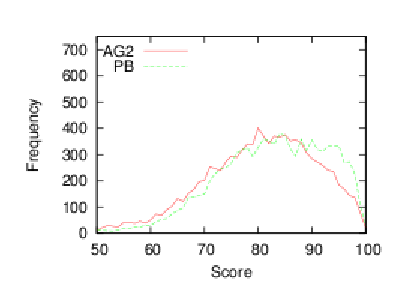
\includegraphics[width=4.5cm]{fr-v-sc-msvl.eps}
            
            Medium dynamism: $\sigma=0.15, \lambda=0.015$
            
            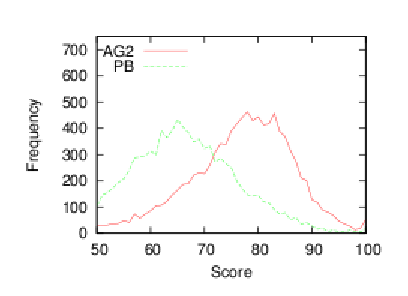
\includegraphics[width=4.5cm]{fr-v-sc-msmi.eps}
            
            High dynamism: $\sigma=2, \lambda=0.2$
            
            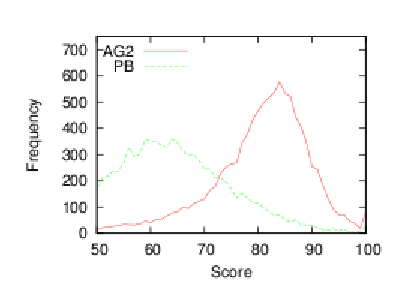
\includegraphics[width=4.5cm]{fr-v-sc-msvh.eps}
            }}
          \end{center}
      \end{minipage}
      \begin{minipage}{8.5cm}
        We ran KEYS 1000 times for each combination of {very low, medium, very high} dynamism and {plan-based, agile 2} prioritization policy. The findings are summarized in \S{RESULTS}. Several majority case effects deserve note:
        \vspace{-0.8em}
        \begin{verysmallitem}
        \item Criticality Modifier: Never chosen in more than $1\%$ of the cases.
        \item Initial Known$/$Inter-Dependency: Never chosen in $>50\%$ of the runs.
        \item Team Size: Never $<5$ team members.
        \item For Agile 2:
          \vspace{-0.7em}
          \begin{verysmallitem}
          \item Size: The smallest size was chosen in $72\%-100\%$ of the runs.
          \item Culture: The upper bins were chosen in $72\%-80\%$ of the runs where dynamism was a factor.
          \item Team Size: Should be 5 - 17 for medium and very high dynamism.
          \end{verysmallitem}
        \end{verysmallitem}

\vspace{-0.8em}
The 1000 runs of KEYS shows that many
results are very similar (e.g. all the Agile 2
          results offer nearly the same pattern). 
KEYS shows that there are two major divisions of 
its 10-dimensional space: very high criticality 
and very small team size. We ran 10,000 
simulations in the union of these two divisions
      \end{minipage}
    }

 (shown above). The median score of Agile 
2 is shows stability under changing dynamism, while 
the median score of Plan-Based falls  as dynamism increases. We see that the median score of Agile 2 is equal to or greater than the median score of Plan-Based development.

    \vspace{3mm}
    We conclude that in the general case, Agile 2 out performs Plan-Based development. Only rarely does Plan-Based out perform Agile 2.
    \vspace{-0.1em}
\end{comment}
\end{kasten}

\begin{kasten}
    \section*{ \hspace{0.1cm} {\color{red} \underline{FOR MORE INFORMATION}}}
    \vspace{-0.5em}
    \normalsize{
      Aaron Riesbeck (\url{aaron.riesbeck@gmail.com})\\
      Adam Brady (\url{adam.m.brady@gmail.com})\\
      Tim Menzies Ph.D. (\url{tim@menzies.us})\\
    }
    \vspace{-0.5em}
\end{kasten}

\begin{kasten}
    \section*{ \hspace{0.1cm} {\color{red} \underline{References}}}
    \vspace{-0.5em}
    \normalsize{
      \begin{enumerate}
      \item J. Eisenstein and R. Davis. Visual and linguistic information in gesture classification. In ICMI, pages 113-120, 2004.
      \item R. J. Larsen and M. L. Marx. An Introduction to Mathematical Statistics and Its Applications, Third Edition. Prentice Hall, 2001.
      \item I. H. Witten and E. Frank. Data Mining: Practical Machine Learning Tools and Techniques with Java Implementations. Morgan Kaufmann, 1999.
      \end{enumerate}
    }
\end{kasten}
